% CSc 8830 -- Computer Vision, Module 2
% Steps 1-3 (calibration, measurement, validation) and the two-camera theory.
%
% Compiles with pdflatex (no external tools, no bibliography):
%     pdflatex report.tex && pdflatex report.tex
% Figures live in ./figures/ and are copies of the pipeline's own output.
\documentclass[11pt,a4paper]{article}

\usepackage[T1]{fontenc}
\usepackage[utf8]{inputenc}
\usepackage[margin=1in]{geometry}
\usepackage{amsmath}
\usepackage{graphicx}
\usepackage{booktabs}
\usepackage{tabularx}
\newcolumntype{L}{>{\raggedright\arraybackslash}X}
\usepackage{longtable}
\usepackage{caption}
\usepackage{subcaption}
\usepackage[colorlinks=true,linkcolor=black,urlcolor=blue]{hyperref}
\usepackage{float}   % [H]: every table and figure stays where it is written

% The one floating table (Table 4) should reach the top of a page rather than
% be deferred onto a page of its own.
\renewcommand{\topfraction}{0.85}
\renewcommand{\floatpagefraction}{0.9}

\setlength{\emergencystretch}{3em}

\newcommand{\px}{\,\mathrm{px}}
\newcommand{\mm}{\,\mathrm{mm}}

\title{Camera Calibration and Real-World Measurement\\
       \large Module 2: Steps 1--3 and Theory}
\author{Raghuveer Gummadi \\ \small CSc 8830: Computer Vision}
\date{\today}

\begin{document}
\maketitle

\section*{Code repository}

\begin{center}
\url{https://github.com/RagDoll95/CSC8830_Assignments}
\end{center}

\noindent
All code, captured images and logged measurements are in that repository. The
Module 2 code is under \texttt{week\_2/module2/} (calibration, measurement,
validation) and the web application that demonstrates it is at the repository
root under \texttt{app/}, served by
\texttt{week\_2/.venv/bin/python app/app.py}. The three Module 2 pages are
\texttt{/module-2/} (calibration), \texttt{/module-2/measure} (click two points
on a photo at a known distance) and \texttt{/module-2/records} (the logged
measurements and error statistics). Per-script usage is documented in
\texttt{week\_2/module2/README.md} and in the header of each script.

\section{Step 1 --- Camera calibration}

A smartphone camera was calibrated with OpenCV's built-in tools by Zhang's
multi-plane method. A $9 \times 6$ inner-corner checkerboard with a measured
square size of $24.9\mm$ was photographed 24 times in varied orientations.
Corners were located with \texttt{cv2.findChessboardCorners} and refined to
sub-pixel accuracy with \texttt{cv2.cornerSubPix}; the camera model was then
fitted with \texttt{cv2.calibrateCamera}, which minimises total reprojection
error over the intrinsics, the distortion coefficients and the per-view pose.
Focus, exposure and zoom were locked for the whole set and every image was
captured at one resolution --- the same resolution used in Steps 2 and 3.

The recovered camera matrix and distortion coefficients are

\begin{equation}
K =
\begin{bmatrix}
3336.69 & 0 & 1496.68 \\
0 & 3335.58 & 2020.27 \\
0 & 0 & 1
\end{bmatrix},
\qquad
\mathbf{d} =
\begin{bmatrix}
0.2231 \\ -1.3758 \\ 0.00058 \\ -0.00081 \\ 2.7090
\end{bmatrix},
\end{equation}

\noindent
in the ordering $(k_1, k_2, p_1, p_2, k_3)$. Since $f$ and $c$ are in pixels,
$K$ is valid only at the $3024 \times 4032$ resolution it was fitted at.
Table~\ref{tab:calib} collects the fit and Figure~\ref{fig:overlays} shows the
detected corners on the best- and worst-fitting views.

\begin{table}[H]
\centering
\caption{Calibration summary.}
\label{tab:calib}
\begin{tabular}{lr}
\toprule
Quantity & Value \\
\midrule
Images used                        & 24 \\
Pattern (inner corners)            & $9 \times 6$ \\
Square size                        & $24.9\mm$ \\
Resolution                         & $3024 \times 4032$ \\
$f_x$                              & $3336.69\px$ \\
$f_y$                              & $3335.58\px$ \\
$c_x$                              & $1496.68\px$ \\
$c_y$                              & $2020.27\px$ \\
$f_y/f_x$                          & $0.99967$ \\
Overall RMS reprojection error     & $1.863\px$ \\
Median per-image RMS               & $0.581\px$ \\
\bottomrule
\end{tabular}
\end{table}

\begin{figure}[H]
\centering
\begin{subfigure}[t]{0.40\textwidth}
  \centering
  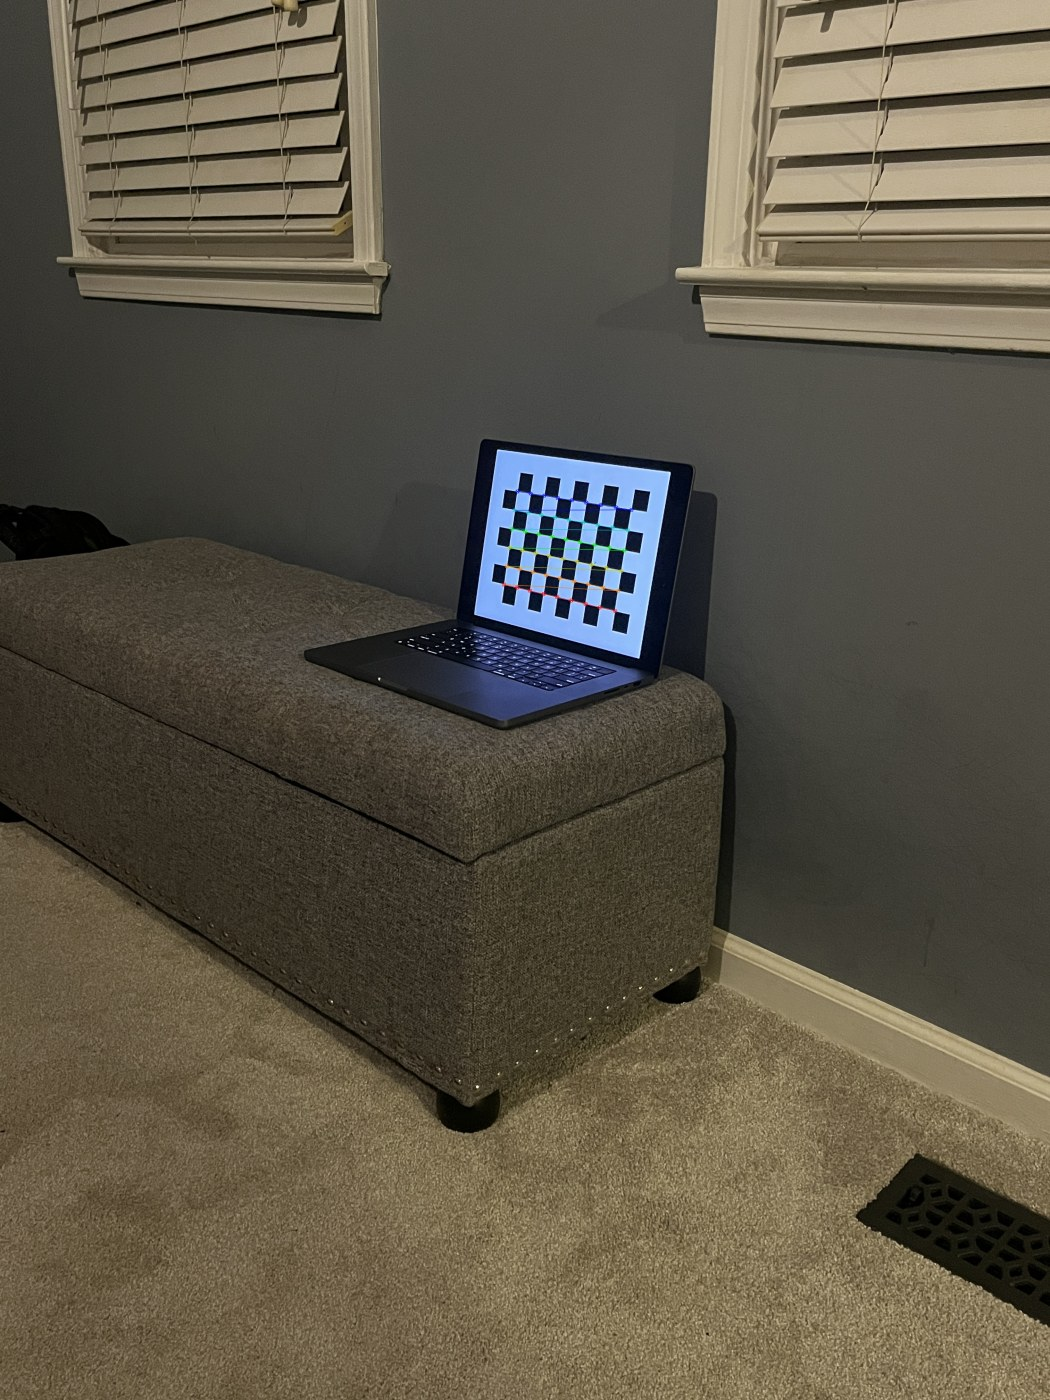
\includegraphics[width=\textwidth]{figures/calib_best.jpeg}
  \caption{\texttt{IMG\_3913}, RMS $0.364\px$.}
\end{subfigure}
\hfill
\begin{subfigure}[t]{0.40\textwidth}
  \centering
  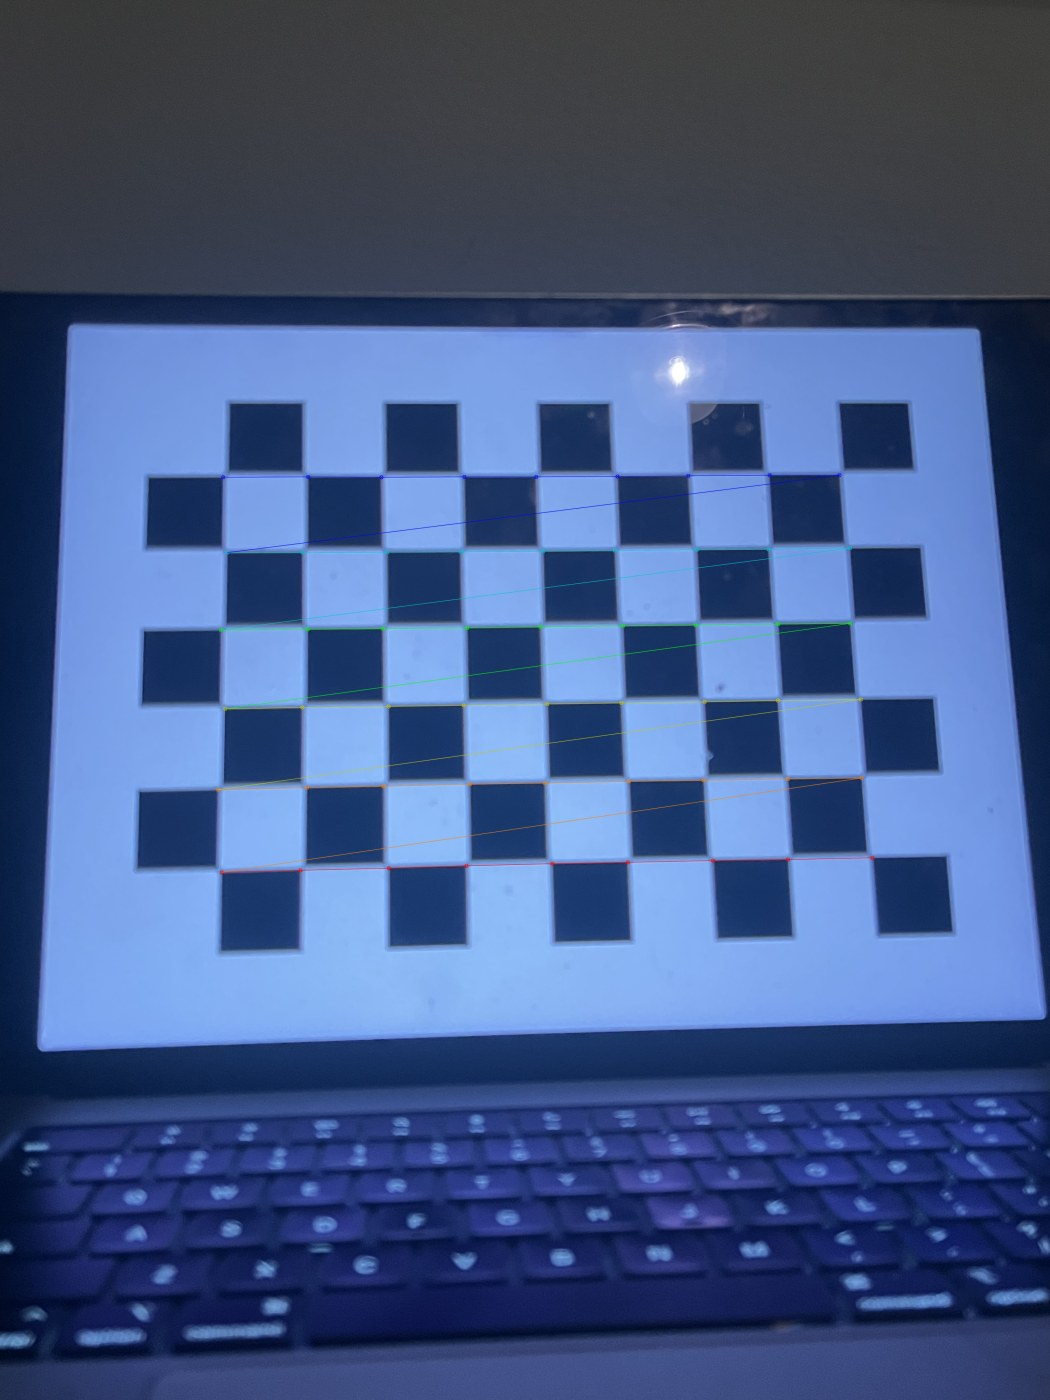
\includegraphics[width=\textwidth]{figures/calib_worst.jpeg}
  \caption{\texttt{IMG\_3921}, RMS $7.475\px$.}
\end{subfigure}
\caption{Detected corner overlays for the best and worst of the 24 calibration
views. Twenty of the 24 images fit below $1\px$ (median $0.533\px$); four land
between $1.22$ and $7.48\px$ and pull the overall RMS above the median.}
\label{fig:overlays}
\end{figure}

\section{Step 2 --- Real-world dimensions from perspective projection}

Under the pinhole model a point $P = (X, Y, Z)$ in camera coordinates projects
to

\begin{equation}
u = f_x \frac{X}{Z} + c_x, \qquad v = f_y \frac{Y}{Z} + c_y .
\label{eq:forward}
\end{equation}

A single image cannot recover $P$, since every point on the ray through $(u,v)$
maps to the same pixel. Supplying the object distance $Z$ independently removes
that one unknown and makes Equation~\ref{eq:forward} invertible:

\begin{equation}
X = (u - c_x)\frac{Z}{f_x}, \qquad Y = (v - c_y)\frac{Z}{f_y} .
\label{eq:backproject}
\end{equation}

A dimension between two selected points $p_1$ and $p_2$ lying on a common plane
at depth $Z$ is then the Euclidean distance between their backprojections,

\begin{equation}
L = \lVert P_2 - P_1 \rVert
  = Z \sqrt{ \left(\frac{\Delta u}{f_x}\right)^{\!2}
           + \left(\frac{\Delta v}{f_y}\right)^{\!2} } ,
\label{eq:length}
\end{equation}

\noindent
which for an axis-aligned span collapses to the familiar

\begin{equation}
W = \Delta u \frac{Z}{f_x}, \qquad H = \Delta v \frac{Z}{f_y} .
\label{eq:wh}
\end{equation}

Width, height and diagonal therefore all come from Equation~\ref{eq:length} by
one code path. Two implementation points matter. Both endpoints must lie at the
same depth $Z$; measuring across a face that recedes from the camera violates
the assumption regardless of calibration accuracy. And lens distortion is
removed from the two selected points only, with
\texttt{cv2.undistortPoints}, which returns \emph{normalised} coordinates
--- already $X/Z$ and $Y/Z$ --- so the dimension is
$Z \cdot \lVert \Delta(\text{normalised}) \rVert$ with no further division by
$f_x$.

The script is \texttt{week\_2/module2/measurement/geometry.py}; running it
directly executes its self-tests (pinhole round trip, distortion path, the $Z$
and resolution guards, and $K$ rescaling).

\section{Step 3 --- Validation experiment}

Twenty object measurements were validated against ruler ground truth. Ground
truth was recorded \emph{before} imaging. Both the object and the measured
dimension were varied: 15 diagonals and 5 widths, over ground-truth sizes from
$77$ to $413\mm$. Nineteen measurements were taken at a nominal
$Z = 2000\mm$, satisfying the requirement that the object be at least
$2$ metres from the camera, and one at $Z = 1000\mm$. Each row stores the two
full-resolution pixel coordinates alongside the result, so
\texttt{analyze.py --recompute} re-derives every logged value from its pixels
(agreeing to within $0.005\mm$). Figure~\ref{fig:meas} shows two of the
annotated measurements, Table~\ref{tab:meas} lists all twenty, and
Table~\ref{tab:stats} and Figure~\ref{fig:diagnostics} report the error
statistics over them.

\begin{figure}[H]
\centering
\begin{subfigure}[t]{0.47\textwidth}
  \centering
  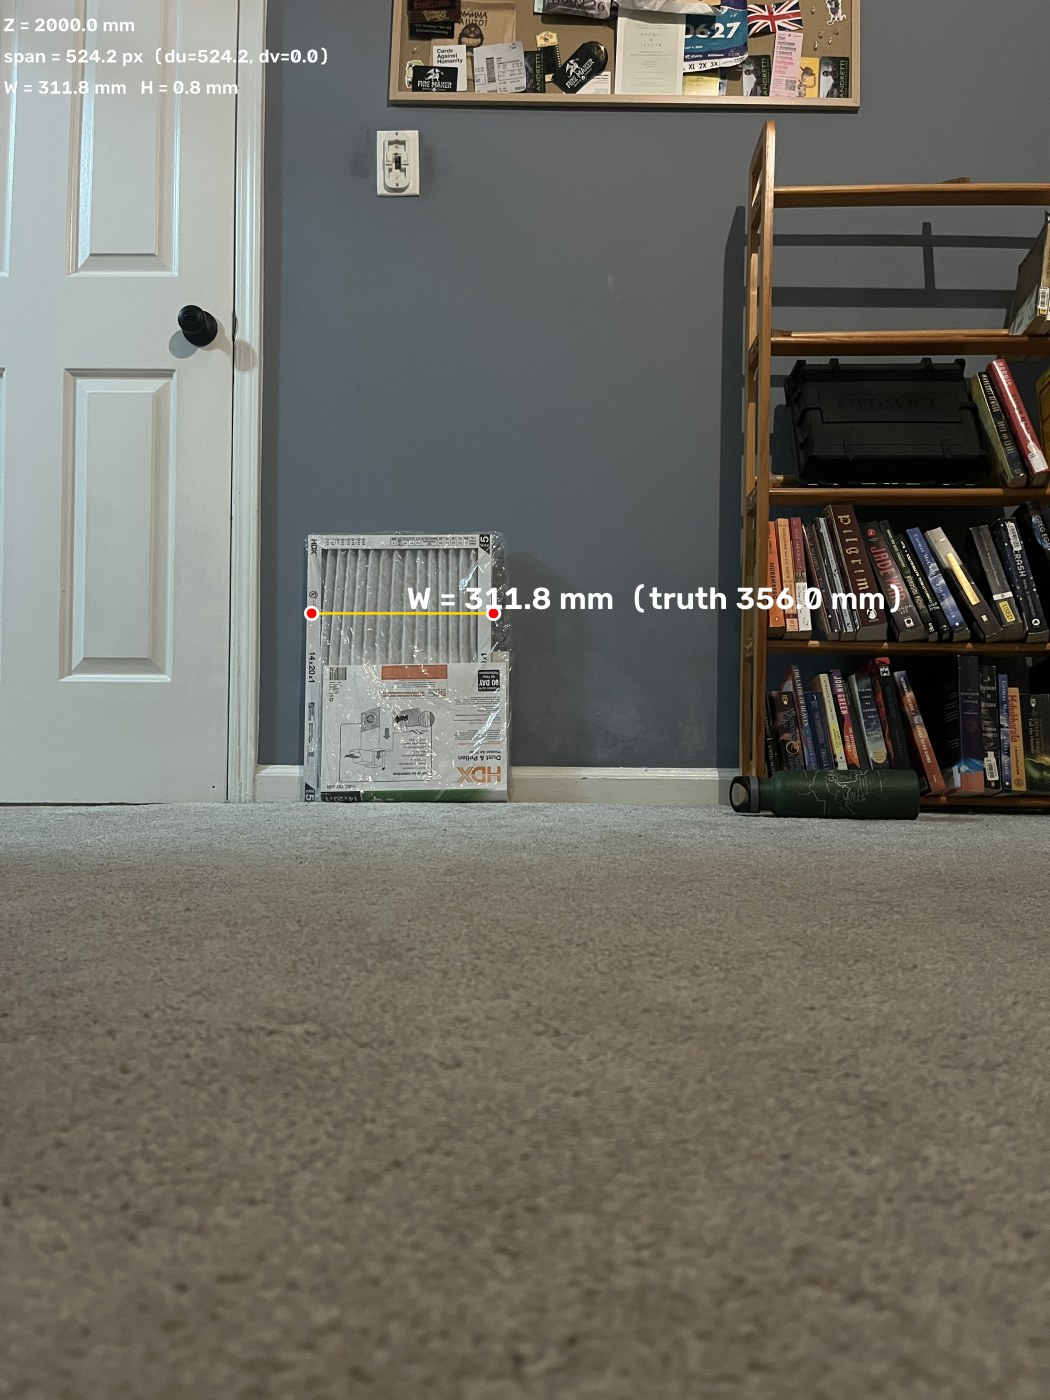
\includegraphics[trim=0 420 0 70,clip,width=\textwidth]{figures/meas_air_filter.jpg}
  \caption{Air filter, $W$: measured $311.8\mm$ against $356.0\mm$.}
\end{subfigure}
\hfill
\begin{subfigure}[t]{0.47\textwidth}
  \centering
  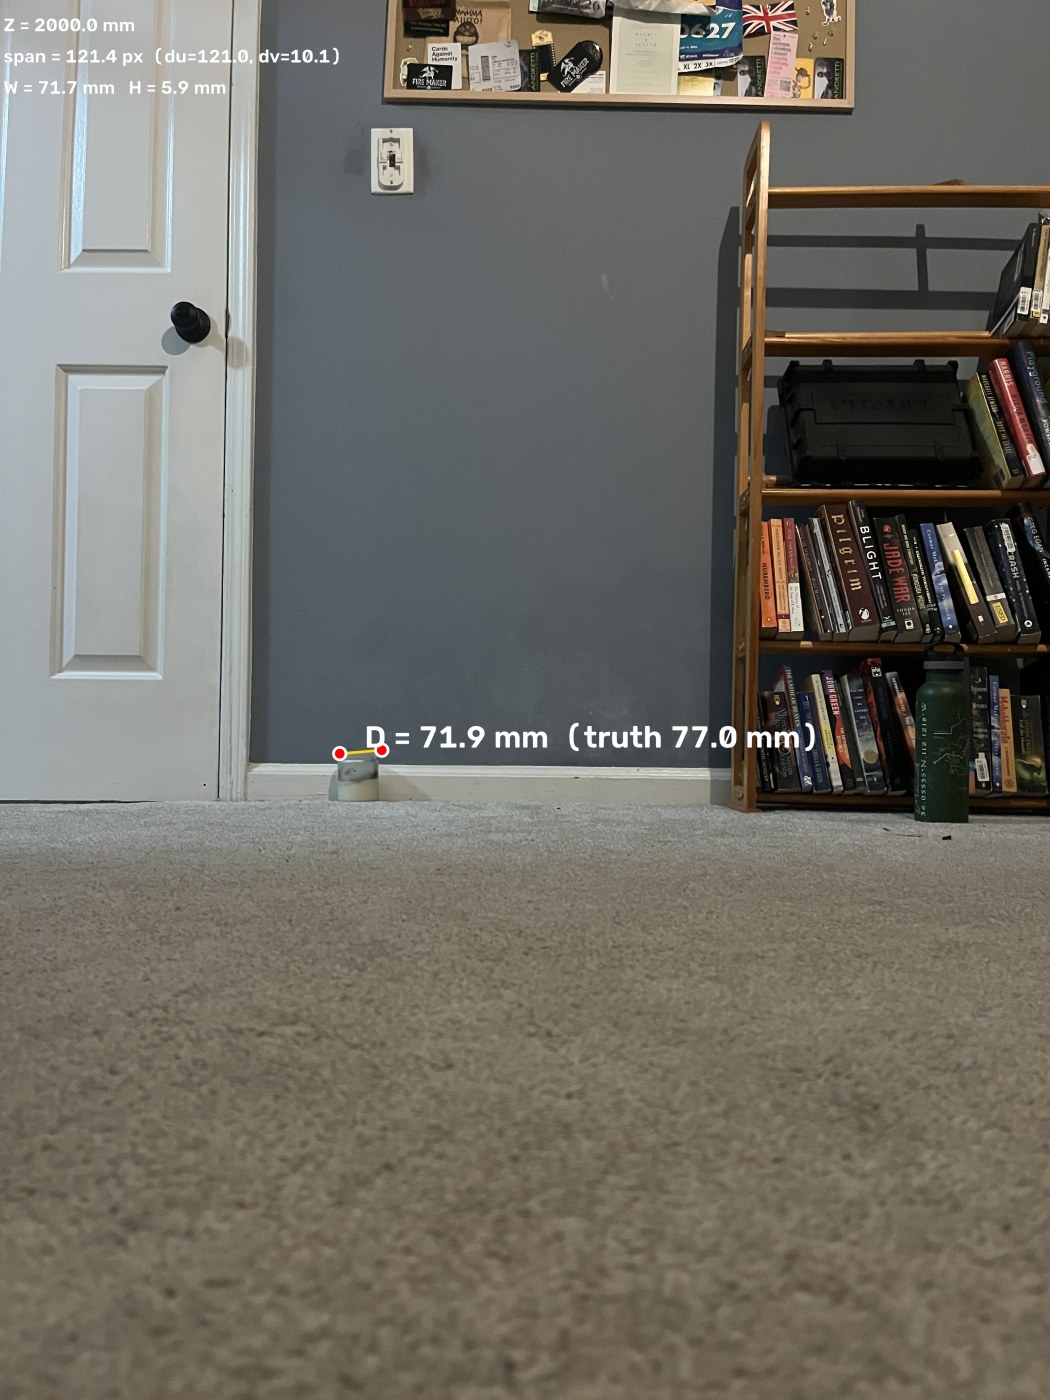
\includegraphics[trim=0 420 0 70,clip,width=\textwidth]{figures/meas_candle.jpg}
  \caption{Candle, $D$: measured $71.9\mm$ against $77.0\mm$.}
\end{subfigure}
\caption{Two of the 20 recorded measurements, at opposite ends of the size
range.}
\label{fig:meas}
\end{figure}

\begin{longtable}{rllrrrrr}
\caption{The 20 validation measurements. Error is
$\text{measured} - \text{truth}$.}
\label{tab:meas} \\
\toprule
id & object & dim & $Z$ (mm) & truth (mm) & meas (mm) & err (mm) & err (\%) \\
\midrule
\endfirsthead
\toprule
id & object & dim & $Z$ (mm) & truth (mm) & meas (mm) & err (mm) & err (\%) \\
\midrule
\endhead
\bottomrule
\endfoot
1 & Mac & D & 1000 & 356.0 & 317.7 & -38.3 & -10.76 \\
2 & Paperback book & D & 2000 & 210.0 & 198.7 & -11.3 & -5.40 \\
3 & Water bottle & D & 2000 & 277.0 & 259.9 & -17.1 & -6.19 \\
4 & Hydroflask & D & 2000 & 130.0 & 168.8 & +38.8 & +29.84 \\
5 & Headphone case & W & 2000 & 150.0 & 149.4 & -0.6 & -0.41 \\
7 & Game controller & D & 2000 & 150.0 & 120.9 & -29.1 & -19.41 \\
8 & clothes hangar & D & 2000 & 413.0 & 360.3 & -52.7 & -12.75 \\
9 & Hardback book & D & 2000 & 160.0 & 144.9 & -15.1 & -9.45 \\
10 & Tissue box & D & 2000 & 231.0 & 227.3 & -3.7 & -1.60 \\
11 & Candle & D & 2000 & 77.0 & 71.9 & -5.1 & -6.58 \\
12 & clothing iron & D & 2000 & 299.0 & 265.1 & -33.9 & -11.32 \\
13 & Climbing shoes & D & 2000 & 229.0 & 204.2 & -24.8 & -10.82 \\
14 & Sketchbook & W & 2000 & 257.0 & 240.6 & -16.4 & -6.38 \\
15 & Duct Tape & D & 2000 & 146.0 & 127.0 & -19.0 & -13.02 \\
16 & Glasses case & D & 2000 & 169.0 & 143.9 & -25.1 & -14.82 \\
18 & Power supply unit & W & 2000 & 168.0 & 155.3 & -12.7 & -7.54 \\
19 & Air filter & W & 2000 & 356.0 & 311.8 & -44.2 & -12.42 \\
20 & Mouse & W & 2000 & 112.0 & 95.6 & -16.4 & -14.63 \\
21 & tennis racket & D & 2000 & 387.0 & 340.2 & -46.8 & -12.08 \\
22 & paperback book 2 & D & 2000 & 200.0 & 180.7 & -19.3 & -9.66 \\
\end{longtable}

\begin{table}[H]
\centering
\caption{Error statistics over the 20 measurements.}
\label{tab:stats}
\begin{tabular}{lr}
\toprule
Statistic & Value \\
\midrule
Measurements, $n$                       & 20 \\
Ground-truth size range                 & $77.0$--$413.0\mm$ \\
Distance range                          & $1000$--$2000\mm$ \\
\midrule
Mean signed error (bias)                & $-19.636\mm$ \\
Standard deviation of error             & $19.914\mm$ \\
MAE                                     & $23.515\mm$ \\
RMSE                                    & $27.610\mm$ \\
\midrule
Mean signed percent error               & $-7.771\%$ \\
MAPE                                    & $10.755\%$ \\
Std.\ deviation of percent error        & $9.948\%$ \\
\midrule
Most negative error                     & $-52.670\mm$ (id 8) \\
Most positive error                     & $+38.790\mm$ (id 4) \\
Standard error of the mean              & $4.453\mm$ \\
$95\%$ CI on mean signed error          & $[-28.364, -10.908]\mm$ \\
\midrule
$\mathrm{corr}(\text{size}, \text{signed error})$  & $-0.721$ \\
$\mathrm{corr}(Z, \text{percent error})$           & $+0.071$ \\
\bottomrule
\end{tabular}
\end{table}

\begin{figure}[H]
\centering
\begin{subfigure}[t]{\textwidth}
  \centering
  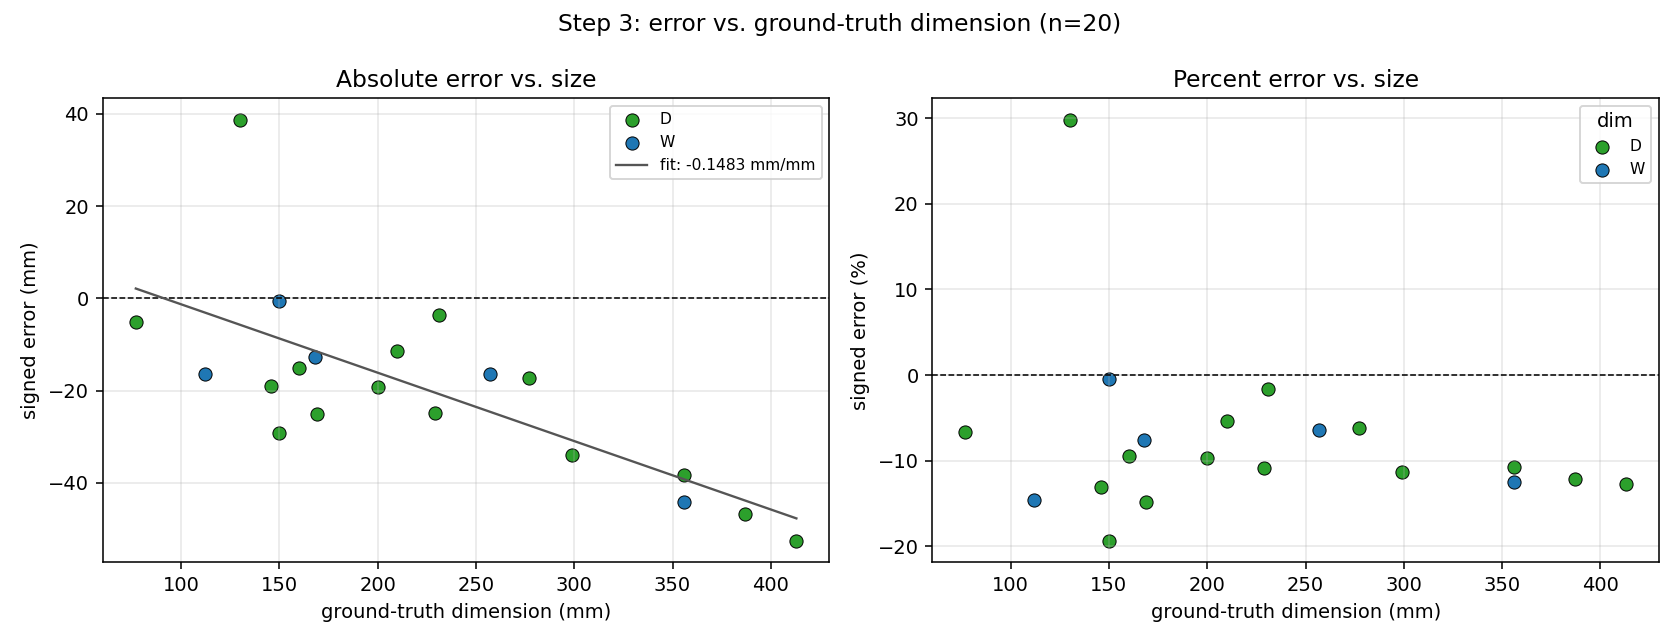
\includegraphics[width=\textwidth]{figures/error_vs_size.png}
  \caption{Error against ground-truth size, in millimetres and in percent.}
\end{subfigure}

\vspace{0.9em}
\begin{subfigure}[t]{\textwidth}
  \centering
  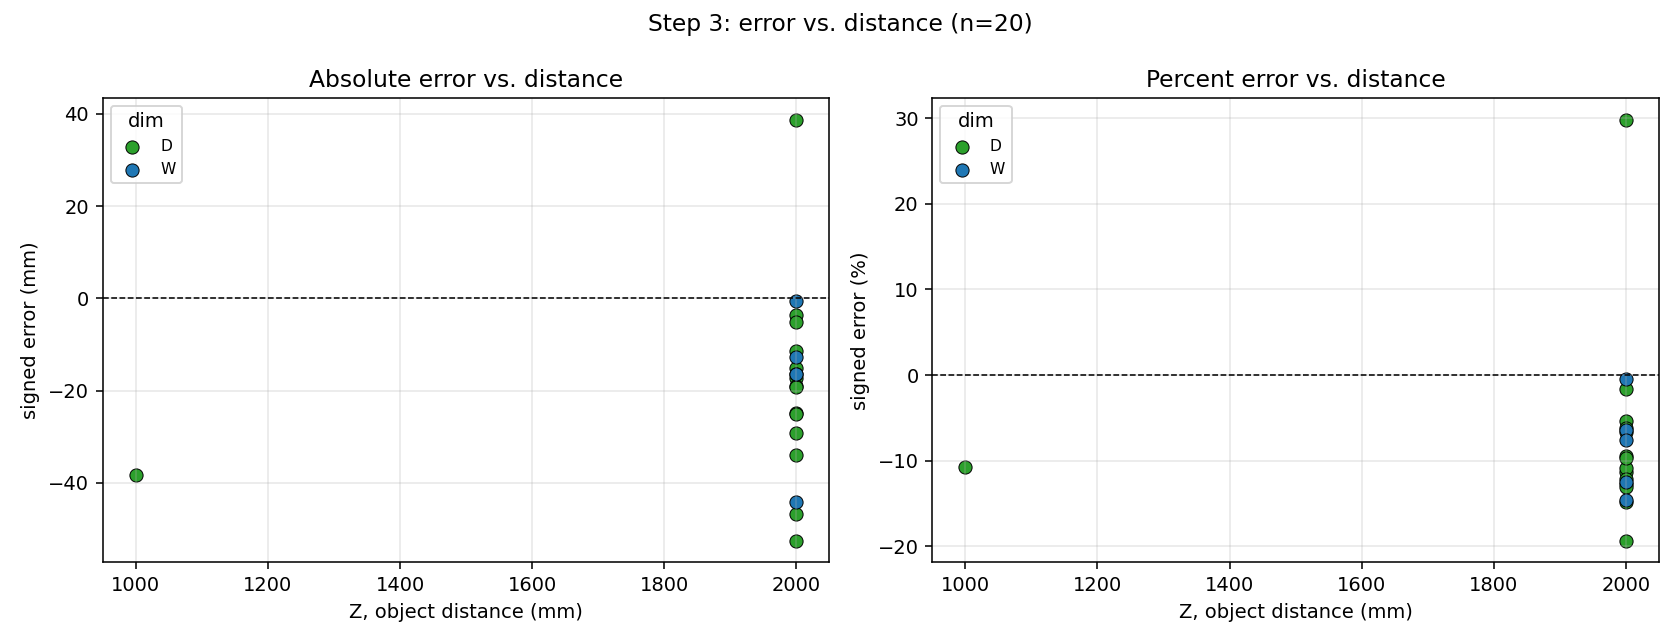
\includegraphics[width=\textwidth]{figures/error_vs_Z.png}
  \caption{Error against object distance; all but one measurement was taken at
  $Z = 2000\mm$.}
\end{subfigure}

\vspace{0.9em}
\begin{subfigure}[t]{0.62\textwidth}
  \centering
  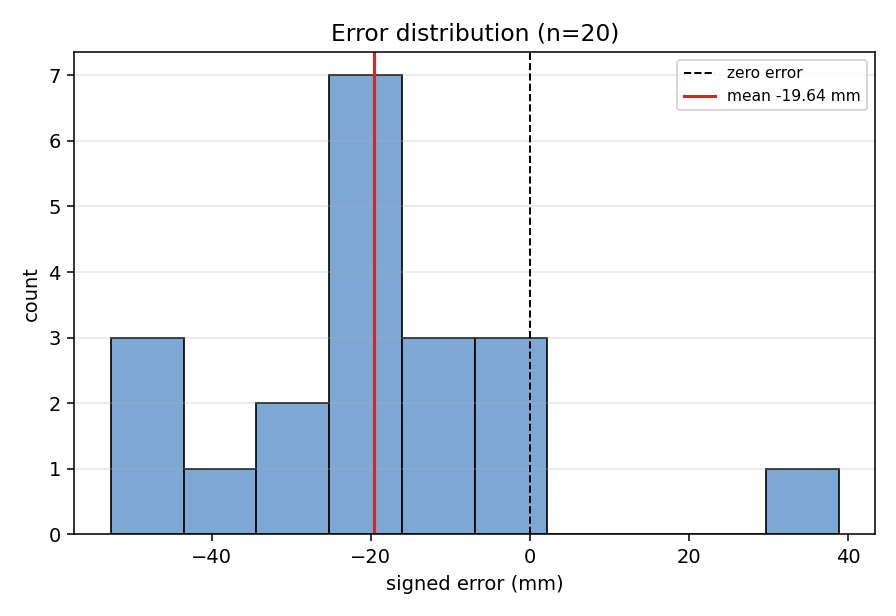
\includegraphics[width=\textwidth]{figures/error_distribution.png}
  \caption{Distribution of percent error.}
\end{subfigure}
\caption{Error statistics of the 20 validation measurements.}
\label{fig:diagnostics}
\end{figure}

\section{Theory --- Relating the image of a point in two cameras}

Camera 1 is static; camera 2 sits at some distance from it and at an oblique
orientation. A point $P = (X, Y, Z)$ lies in the field of view of both. What
follows relates $x_1$, the image of $P$ in camera 1, to $x_2$, its image in
camera 2.

\subsection{Assumptions}

\begin{enumerate}
  \item \textbf{Ideal pinhole projection.} Both images are undistorted first,
        using the distortion coefficients from Step 1. After correction the
        residual departure from an ideal pinhole is below the
        corner-localisation noise, so modelling it further would add
        parameters without reducing error.
  \item \textbf{Both cameras are calibrated.} $K_1$ and $K_2$ are known from a
        Zhang calibration as in Step 1. If one phone captures both views then
        $K_1 = K_2 = K$, which removes half the unknown intrinsics; that is the
        case here.
  \item \textbf{Zero skew, square pixels.} The Step 1 fit gives $f_y/f_x$
        within $0.03\%$ of unity and CMOS pixel axes are orthogonal by
        construction, so the skew term in $K$ is set to zero rather than
        estimated.
  \item \textbf{Rigid relative pose.} $R$ and $\mathbf{t}$ are constant for the
        pair of exposures. From a rig, the rig does not flex; from one phone
        moved by hand, $R$ and $\mathbf{t}$ refer to those two exposures and to
        nothing else.
  \item \textbf{World frame anchored to camera 1.} A free choice of gauge, not
        a physical claim, and the one that makes the algebra clean: camera 1's
        extrinsics become $[\,I \mid \mathbf{0}\,]$, so $P$ in the world frame
        \emph{is} $P$ in camera 1's frame.
  \item \textbf{$P$ has positive depth in both frames.} The chirality
        condition, implied by ``within the FoV of both''. It is what makes the
        projective equalities below correspond to real image points rather
        than to points behind a camera.
  \item \textbf{Static scene.} $P$ does not move between the two exposures ---
        required whenever the views are captured sequentially with one camera.
\end{enumerate}

\subsection{The two projections}

With $\cong$ denoting equality up to a nonzero scale in homogeneous
coordinates, and the world frame on camera 1,

\begin{equation}
x_1 \cong K_1 [\,I \mid \mathbf{0}\,] X = K_1 P,
\qquad
x_2 \cong K_2 [\,R \mid \mathbf{t}\,] X = K_2 (R P + \mathbf{t}),
\label{eq:twoproj}
\end{equation}

\noindent
where $x_1 = (u_1, v_1, 1)^{\!\top}$ and $x_2 = (u_2, v_2, 1)^{\!\top}$ are the
homogeneous image points, $R \in SO(3)$ is camera 2's rotation relative to
camera 1, and $\mathbf{t} = -R\tilde{C}$ with $\tilde{C}$ the centre of camera
2 expressed in camera 1's frame --- so $\mathbf{t}$ is a translation
\emph{in camera 2's frame}, not a displacement in camera 1's. ``Oblique
orientation'' is precisely the statement $R \neq I$, and ``at some distance''
is $\mathbf{t} \neq \mathbf{0}$.

\subsection{Substitution gives the relationship}

The first equation of \eqref{eq:twoproj} inverts to $P = Z\,K_1^{-1} x_1$,
which is the Step 2 backprojection reused: $x_1$ fixes the ray on which $P$
lies and the scalar $Z$ is the one missing quantity. Substituting into the
second and dividing through by $Z$ --- legal because the relation is
projective --- gives

\begin{equation}
\boxed{\;
x_2 \;\cong\; H_\infty\, x_1 \;+\; \frac{\mathbf{e}_2}{Z} \;}
\qquad
H_\infty = K_2 R K_1^{-1},
\qquad
\mathbf{e}_2 = K_2 \mathbf{t},
\label{eq:main}
\end{equation}

\noindent
where $H_\infty$ is the infinite homography and $\mathbf{e}_2$ the epipole in
image 2. In words: the image of $P$ in camera 2 is $x_1$ warped by the rotation
and the two sets of intrinsics, then displaced along the direction of the
epipole by an amount inversely proportional to the depth of $P$. Two
consequences follow. $H_\infty$ is the limit as $Z \to \infty$, so points at
infinity map by $H_\infty$ alone and are unaffected by the baseline --- which
is why distant scenery barely shifts between two views while near objects
shift a lot. And sweeping $Z$ from $0$ to $\infty$ traces a line in image 2,
the epipolar line of $x_1$: a single view cannot recover depth, because the
whole line is consistent with the one observation $x_1$. That is why Step 2
needed a measured $Z$.

\subsection{The depth-free form}

Eliminating $Z$ leaves a relation between the image coordinates alone. Since
$P_2 = RP + \mathbf{t}$, the vectors $P_2$, $\mathbf{t}$ and $RP$ are coplanar,
so the triple product $P_2 \cdot (\mathbf{t} \times RP)$ vanishes. In matrix
form,

\begin{equation}
\boxed{\; x_2^{\!\top} F\, x_1 = 0 \;}
\qquad
F = K_2^{-\top} [\mathbf{t}]_\times R\, K_1^{-1},
\qquad
E = [\mathbf{t}]_\times R = K_2^{\!\top} F K_1,
\label{eq:epipolar}
\end{equation}

\noindent
with $F$ the fundamental matrix, $E$ the essential matrix and
$[\mathbf{t}]_\times$ the skew-symmetric matrix satisfying
$[\mathbf{t}]_\times y = \mathbf{t} \times y$. $F$ has 7 degrees of freedom
(nine entries, less one for scale and one for $\det F = 0$) and $E$ has 5
(three for $R$, three for $\mathbf{t}$, less one for the scale of
$\mathbf{t}$). Because $E$ is unchanged by scaling $\mathbf{t}$, translation is
recoverable from correspondences only up to scale; metric scale requires one
real length in the world, such as a checkerboard square or a tape-measured
baseline $\lVert \mathbf{t} \rVert$.

\subsection{Scalar form}

Writing the rows of $R$ as $r_1^{\!\top}, r_2^{\!\top}, r_3^{\!\top}$ and
$\mathbf{t} = (t_x, t_y, t_z)^{\!\top}$, camera 2's projection is

\begin{equation}
u_2 = f_{x2}\,\frac{r_1^{\!\top}P + t_x}{r_3^{\!\top}P + t_z} + c_{x2},
\qquad
v_2 = f_{y2}\,\frac{r_2^{\!\top}P + t_y}{r_3^{\!\top}P + t_z} + c_{y2}.
\label{eq:scalar}
\end{equation}

\noindent
The denominator $r_3^{\!\top}P + t_z$ is the depth of $P$ in camera 2's frame.
This form makes concrete what the matrix form hides: the mapping is nonlinear
in $P$, and the nonlinearity sits entirely in that one shared denominator.
Parametrising $R$ by ZYZ Euler angles, $R(\psi, \theta, \phi) = R_z(\phi)
R_y(\theta) R_z(\psi)$, the complete set of static unknowns relating the two
cameras is $(\psi, \theta, \phi, t_x, t_y, t_z)$ --- six numbers, of which five
are recoverable from correspondences and the sixth, the scale of $\mathbf{t}$,
needs one external length.

\subsection{Parameters and variables}

Table~\ref{tab:params} lists every symbol used above --- whether it is a
static parameter of the pair of cameras, a quantity derived from those, or a
per-point variable --- and how each one is measured or computed.

\begin{table}[t]
\caption{Every quantity in Equations~\eqref{eq:main}--\eqref{eq:scalar}, and
how each is obtained.}
\label{tab:params}
\small
\begin{tabularx}{\textwidth}{@{}llLL@{}}
\toprule
Symbol & Type & Meaning & How obtained \\
\midrule
$K_1, K_2$ & static & Intrinsic matrix of each camera & Zhang calibration,
Step 1. Equal if one phone takes both views. \\
$\mathbf{d}_1, \mathbf{d}_2$ & static & Distortion coefficients & Step 1;
applied to undistort both images before anything above is used. \\
$R$ & static & Relative rotation, camera 1 $\to$ camera 2 &
\texttt{cv2.stereoCalibrate} with the board visible in both views, or
\texttt{cv2.recoverPose} / decomposition of $E$. \\
$\mathbf{t}$ & static & Relative translation, $\mathbf{t} = -R\tilde{C}$ & As
for $R$. From $E$ alone it is direction-only; metric scale needs one known
length. \\
$\lVert \mathbf{t} \rVert$ & static & Baseline & Measured with a ruler, or
fixed by the known square size in \texttt{stereoCalibrate}. \\
$\psi, \theta, \phi$ & static & ZYZ Euler angles of $R$ & Extracted from $R$
via \texttt{cv2.Rodrigues} and an Euler conversion. \\
$H_\infty$ & derived & Infinite homography $K_2 R K_1^{-1}$ & Computed from
$K_1, K_2, R$. \\
$\mathbf{e}_2$ & derived & Epipole in image 2, $K_2\mathbf{t}$ & Computed from
$K_2, \mathbf{t}$. \\
$F$ & derived & Fundamental matrix & From $K_1, K_2, R, \mathbf{t}$, or
estimated directly from $\geq 8$ correspondences
(\texttt{cv2.findFundamentalMat}). \\
$E$ & derived & Essential matrix $[\mathbf{t}]_\times R$ &
$K_2^{\!\top} F K_1$, or \texttt{cv2.findEssentialMat} from $\geq 5$
correspondences. \\
$x_1, x_2$ & variable & Image coordinates of $P$ in each view & Measured:
feature detection and matching, or manual selection. \\
$P = (X,Y,Z)$ & variable & The scene point & Unknown; recovered by
triangulation once $x_1, x_2, R, \mathbf{t}$ are known. \\
$Z$ & variable & Depth of $P$ in camera 1's frame & Triangulated from the two
views, or measured with a tape as in Step 3. \\
\bottomrule
\end{tabularx}
\end{table}

\subsection{Degenerate cases}

\begin{description}
  \item[Pure rotation, $\mathbf{t} = \mathbf{0}$.] Equation~\eqref{eq:main}
    collapses to $x_2 \cong H_\infty x_1$ with no depth term: every point maps
    by one homography however far away it is, so depth is unrecoverable and $F$
    is undefined. Panning a phone on a tripod yields no depth information, no
    matter how many frames are taken.
  \item[$P$ on a plane.] If all points satisfy $n^{\!\top}P = d$, then $Z$ can
    be eliminated through the plane equation and the mapping becomes the
    plane-induced homography $H = K_2(R + \mathbf{t}n^{\!\top}\!/d)K_1^{-1}$,
    again independent of per-point depth. This is the same coplanarity
    degeneracy that makes one checkerboard view insufficient for calibration,
    and why Zhang's method needs several orientations.
  \item[$P$ on the baseline.] Then $x_1 \cong \mathbf{e}_1$ and
    $x_2 \cong \mathbf{e}_2$, Equation~\eqref{eq:epipolar} is satisfied
    identically, the correspondence carries no information and triangulation is
    singular.
\end{description}

\subsection{Inverting the derivation: triangulation}

With $x_1, x_2, R, \mathbf{t}$ and both intrinsics known, the two projections
of \eqref{eq:twoproj} give four equations in the three unknowns of $P$.
Writing each as a cross product $x \times (\mathcal{P}X) = \mathbf{0}$ yields a
homogeneous system $A X = \mathbf{0}$, solved by the singular vector of $A$
with the smallest singular value; \texttt{cv2.triangulatePoints} does exactly
this. Real-world dimensions then follow as the Euclidean distance between two
triangulated points, with no tape measure in the pipeline --- which directly
addresses the limitation of Steps 2 and 3, whose accuracy is bounded below by
how well $Z$ can be measured by hand. Metric scale must still enter once, via
$\lVert \mathbf{t} \rVert$ or a known length in the scene.

\end{document}
